%%%%%%%%%%%%% MATLAB %%%%%%%%%%%%%%%%%%
\subsection{MatLab}
\label{matlab}

Da die Verfahren der Regressionsmodelle, wie im vorherigen Abschnitt beschrieben, sehr komplex und aufwendig sind, und deren Umsetzung nur noch durch rechnergestützte Mathematik möglich ist, bietet sich die Nutzung eines hierfür speziell ausgerichteten Software-Tools an.\footnote{Weitere Software-Tools: R, SPSS, KNIME, SAS, uvm.} Die \gls{matlab}-Plattform stellt eine intuitive und zugleich auch interaktive Umgebung für die Modellierung von Funktionen bereit und wird zur Lösung der vorliegenden Problemstellung in der Version \textit{R2016B}\footnote{Testversion für Studenten} verwendet. Im Folgenden soll dem Leser die Software, sowie die von ihr gebotenen Möglichkeiten zur Datenanalyse und Regressionsmodellierung, kurz vorgestellt werden. 

\subsubsection{Allgemein}
\gls{matlab} ist eine von MathWorks Inc. entwickelte Software-Plattform, die 1984 erstmalig kommerziell ausgeliefert und seitdem stetig weiter entwickelt wurde.\seFootcite{Vgl.}{S. 1}{Pietruszka.2014}\seFootcite{Vgl.}{S. 337}{Shardt.2015} Es wird für \gls{ml}, Signal- und Bildverarbeitung, Finanzmathematik, Robotik und viele weitere Anwendungsbereiche genutzt und gilt heute als die verbreitetste Software für Analysen und Designs von Systemen und Produkten.\seFootcite{Vgl.}{S. 1}{Gupta.2014} Darüber hinaus eignet es sich besonders für Data-Mining-Methoden, wie der beispielsweise Regression oder Klassifizierung. Das Portfolio umfasst rechnerunterstützte numerische Berechnungen und Visualisierungen, sowie eine eigene Hochsprache mit Programmierumgebung. Weiterhin werden vorgefertigte spezifische Bibliotheken in Form von Toolboxen angeboten, wie beispielsweise das in dieser Arbeit verwendete \gls{cft} zur Funktionsmodellierung.\seFootcite{Vgl.}{S. 1}{Pietruszka.2014} Dadurch können beispielsweise numerisch aufwendige Verfahren der Regressionanalyse, wie die \textit{nichtparametrische Regression} (siehe \vref{rm}), schnell und interaktiv durchgeführt werden. 

\subsubsection{Regressionsanalyse}

Die \gls{matlab}-Plattform realisiert die Regressionsanalyse in Form der dafür vorgefertigten Bibliothek \gls{cft}. Die Bestandteile und das Verfahren dieser Toolbox soll mit Hilfe der \vref{cft} anhand eines einfachen Beispiel erläutert werden. Hierbei liegen Datenwerte zu der unabhängigen Variable $x$ und der abhängigen Variable $y$ vor, die zunächst den Achsen zugeordnet werden (siehe gelber Kasten oben links). Im nächsten Schritt kann aus einer Vielzahl von Funktionstypen eine passende ausgewählt werden, wie in diesem Fall eine Polynomialfunktion 1. Grades (siehe grüner Kasten), da eine \textit{lineare Regressionsfunktion} vermutet wird. Das \gls{cft} berechnet mit den Methoden der Regressionsanalyse, sprich der Minimierung der Summe der kleinsten Quadrate (vgl. \vref{ra}), die gesuchten Parameter $p1$ und $p2$ der Regressionsfunktion (siehe blauer Kasten). Des weiteren werden auch die zuvor dargestellten Bestimmtheitsmaße $R^2$ und $\overline{R}^2$, die den \textit{Goodness of fit} messen, ausgeben, sodass eine Evaluation des Modells vorgenommen werden kann (siehe roter Kasten). In diesem Fall liegt mit etwa 98\% eine sehr genaue Anpassung des Modells an die Daten vor. Zuletzt kann die resultierende Funktion sowie die Datenpunkte in einem Koordinatensystem betrachtet werden, um auch einen graphische Vorstellung zu erlangen. Das Tool bietet eine intuitive Benutzung, wodurch verschiedene (vermutete) Regressionsmodelle schnell und einfach mit einander verglichen werden können, ohne dabei die aufwendigen und komplexen Rechenmethoden selbst durchführen zu müssen. Neben dieser graphischen Möglichkeit bietet \gls{matlab} auch in der mitgelieferten Programmierumgebung vorgefertigte Funktionen für die Regressionsanalyse, auf die hier jedoch nicht weiter eingegangen wird.

\begin{sidewaysfigure}
\centering
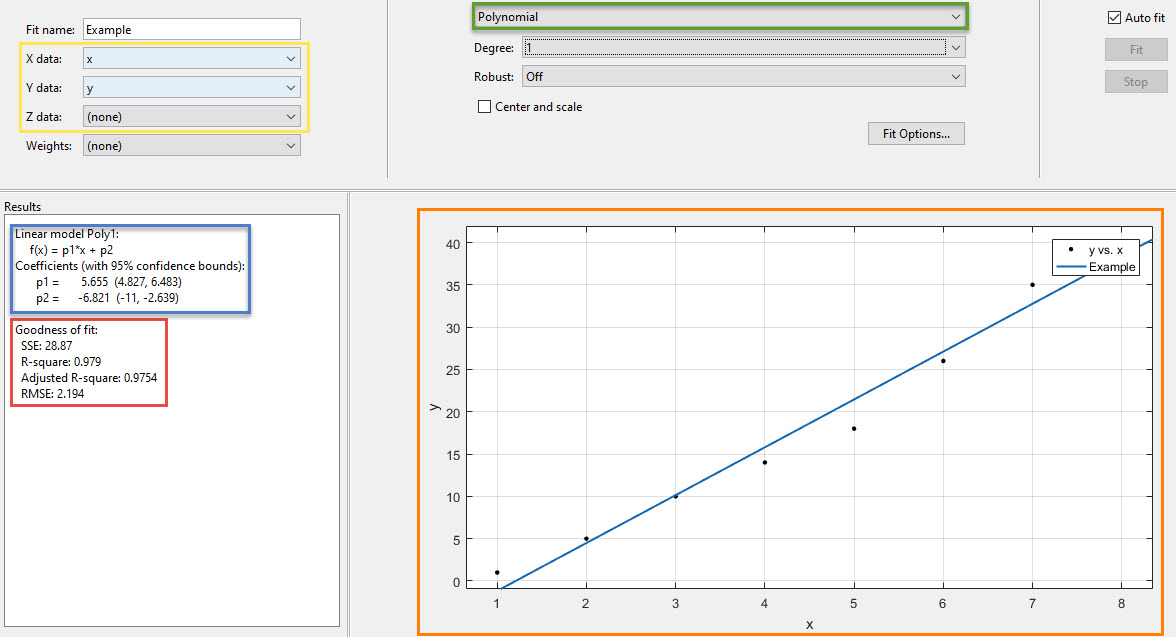
\includegraphics[scale=0.675]{se-wa-jpg/cft}
\caption[Bestandteile des Curve Fitting Tools]{Bestandteile des Curve Fitting Tools\protect\footnotemark}
\label{cft}
\footnotetext{Screenshot aus MATLAB}
\end{sidewaysfigure}
